\addtocontents{toc}{\protect\vspace{10pt}}
\section{Chapter 8: Bayesian statistics}

\learningobjectives{
    \item Specifying and interpreting a prior distribution
    \item Updating a prior distribution to a posterior distribution
    \item Quantifying evidence for a model using the Bayes factor
}

% To add an assignment to the chapter, create a file in the folder "Assignments" and insert the link below

\setcounter{chapter}{8}
\setcounter{section}{1}
\setcounter{question}{0}
\setcounter{hint}{0} % Only for first assignment in chapter

%%%%%%%%%%%%%%%%%%%%%%%%%%%%%%%%%%%%%%%%%%%%%%%%%%%%%%%%%%%%%%%%%%%%%%%%%%%
% Assignment 8.1: Specifying and interpreting a prior distribution
%%%%%%%%%%%%%%%%%%%%%%%%%%%%%%%%%%%%%%%%%%%%%%%%%%%%%%%%%%%%%%%%%%%%%%%%%%%

\rassignment{Specifying and interpreting a prior distribution}

In this final chapter we move away from the traditional statistical methods that you have learned (\concept{confidence intervals} and \concept{p-values}), and introduce a different methodology; Bayesian statistics. Bayesian statistics expresses the most basic idea in learning, namely, that your prior belief in an event is updated to a posterior belief after observing data. By first specifying your prior beliefs, you allow yourself to learn from the data that you have collected, thereby updating your prior belief to a more informed posterior belief. Bayesian statistics is a powerful tool that can help you to update your existing beliefs in the context of new business information. \\

In Bayesian inference, your prior beliefs about a \concept{parameter} are expressed through a \concept{probability distribution}. For example, in tossing a coin, the probability of heads occurring may be defined as a \concept{parameter} $\theta$. Your initial probability distribution (i.e., beliefs) on $\theta$ is called the \concept{prior distribution}, which can be interpreted quite visually. The figure below shows three possible prior distributions for the probability of heads in a coin toss. The area under the curve represents probability.

\begin{center}
    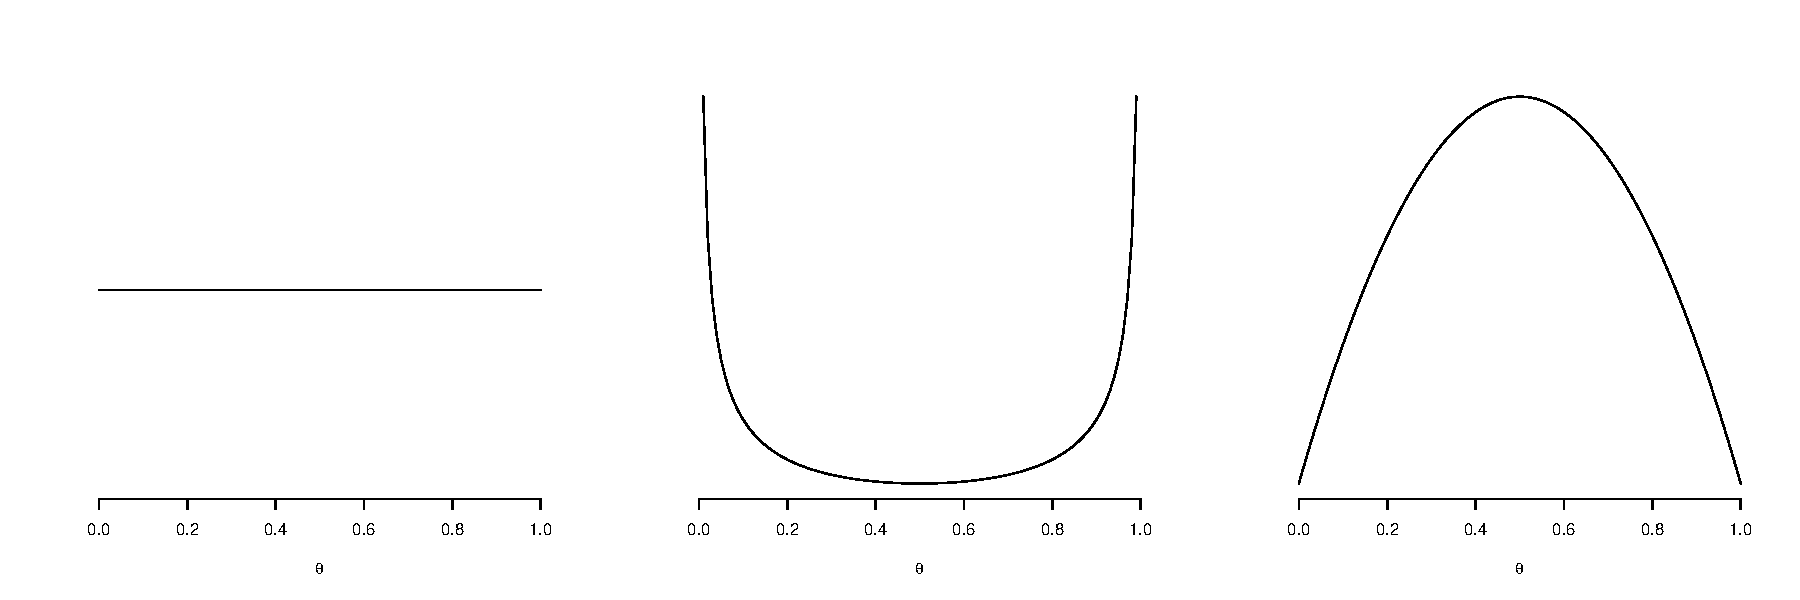
\includegraphics[width=\textwidth]{Files/Images/priorDistributions.pdf}
\end{center}

\question{
    Interpret the three \concept{prior distributions} above and discuss what information about the probability $\theta$ of the coin occurring on heads they incorporate.
}

\twolineanswerbox

\clearpage % Page break

When estimating a proportion (like the probability of heads in a coin toss) you can use the common $Beta(\alpha,\, \beta)$ distribution as a prior distribution on $\theta$ since it is restricted to the range [0, 1]. The $Beta(\alpha,\, \beta)$ distribution has two parameters, $\alpha$ and $\beta$, that have an effect on its shape. By playing around with these parameters, you can create the \concept{prior distribution} that reflects your particular beliefs as accurately as possible. \\

Run the following code in \texttt{R} to create the \concept{prior distribution} shown on the left of the figure above: \\

\codeblock{alpha <- 1 \\
beta <- 1 \\
curve(dbeta(x, alpha, beta), xlab = expression(theta), ylab = \textquotesingle\textquotesingle, yaxt = \textquotesingle n\textquotesingle)}

\question{Recreate the middle and right \concept{prior distributions} from the figure by changing the values for \rcode{alpha} and \rcode{beta} and running the code again. What are the values of $\alpha$ and $\beta$ for these distributions?}

\rcodeanswersmall

\emptyanswerbox{
    Middle: \hspace*{5cm} Right \\
    \\
    $\alpha$: \shortanswerline  \hspace*{2.5cm} $\alpha$: \shortanswerline
    \answerbreak
    $\beta$: \shortanswerline \hspace*{2.5cm} $\beta$: \shortanswerline
}

\question{How would you define a \concept{prior distribution} for $\theta$ if you believed the coin was definitely biased towards heads? And for one that is biased towards tails? Draw these \concept{prior distributions} below.}

\emptyanswerbox{
    \vspace*{-.5cm}
    \hspace*{2.1cm} Biased towards heads: \hspace*{0.65cm} Biased towards tails:
    \vspace*{-7.5pt}
    \begin{center}
        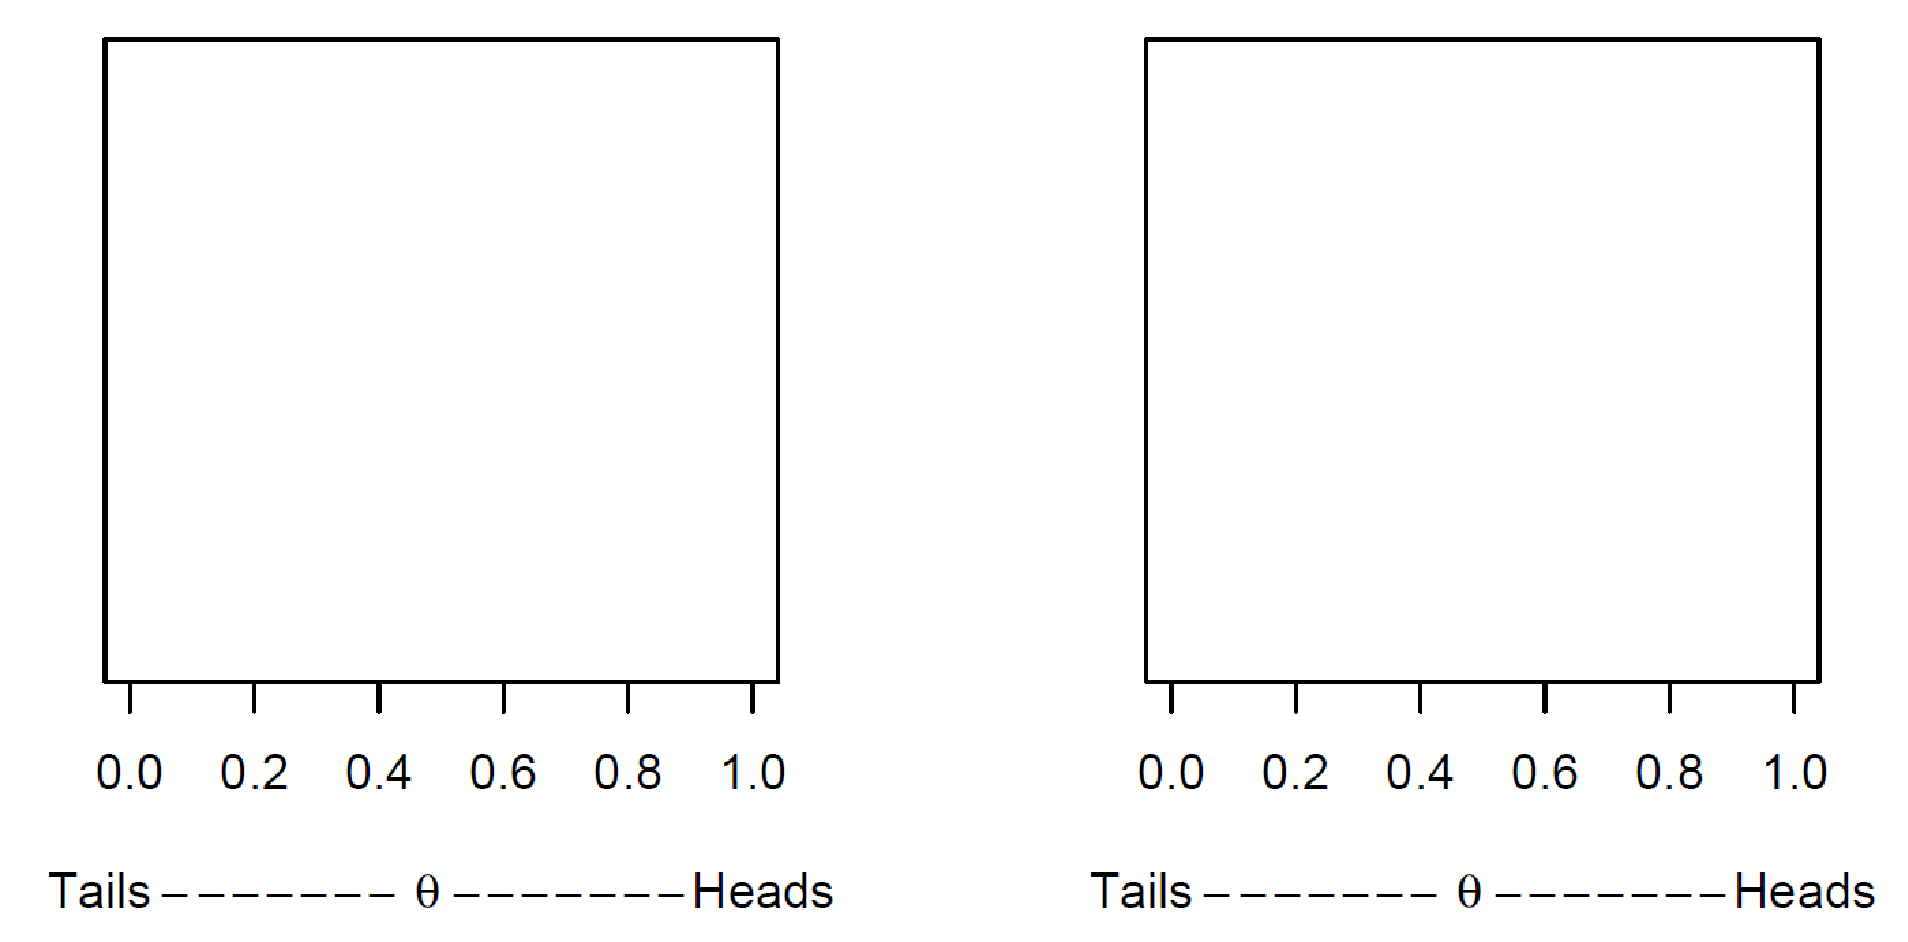
\includegraphics[height=5.3cm]{Files/Images/priorDistributionsAnswerField.pdf}
    \end{center}
}

\clearpage % Page break
\setcounter{section}{8}
\setcounter{subsection}{2}
\setcounter{question}{0}

%%%%%%%%%%%%%%%%%%%%%%%%%%%%%%%%%%%%%%%%%%%%%%%%%%%%%%%%%%%%%%%%%%%%%%%%%%%
% Assignment 8.2: Updating a prior distribution to a posterior distribution
%%%%%%%%%%%%%%%%%%%%%%%%%%%%%%%%%%%%%%%%%%%%%%%%%%%%%%%%%%%%%%%%%%%%%%%%%%%

\rassignment{Updating a prior distribution to a posterior distribution}

Suppose you are the manager of a small store and want to estimate what proportion of your customers leaves the store with a feeling of satisfaction. You give out a questionnaire to 40 people in the store and ask them whether they felt satisfied or not. In a previous enquiry done by you, it was already shown that, on average, 60\% of your customers feels good about the store, with a \concept{standard deviation} of ten percent. Using Bayesian statistics, you are now going to update the information from your previous enquiry with the information from the new questionnaire. \\

\question{What \concept{parameter} does $\theta$ represent in this scenario?}

\hint{Think about what question you are interested in answering.}

\onelineanswerbox

\question{Think of your own $\alpha$ and $\beta$ parameters for the $Beta(\alpha, \,\beta)$ \concept{prior distribution} on $\theta$. Take into account the average percentage from your previous enquiry and incorporate this into your \concept{prior distribution.}}

\emptyanswerbox{
    $\alpha$: \shortanswerline \hspace*{3cm} $\beta$: \shortanswerline
}

\question{Use the \rcode{curve()} function to create a figure of your \concept{prior distribution} in \texttt{R}.}

\rcodeanswertiny

By updating the $Beta(\alpha,\, \beta)$ prior distribution with information that you have collected, you create a \concept{posterior distribution}, which contains both the prior information and the information from the sample. Having observed $k$ successes in a sample of $n$ observations, the \concept{prior parameters} $\alpha$ and $\beta$ are updated to the \concept{posterior parameters} $\alpha + k$ and $\beta + n - k$. \\

In your sample of $n = 40$ questioned customers, $k = 33$ said they felt satisfied when leaving the store. \\

\clearpage % Page break

\question{Write down the \concept{parameters} of the \concept{posterior distribution}.}

\emptyanswerbox{
    $\alpha$: \shortanswerline \hspace*{3cm} $\beta$: \shortanswerline
}

Run the following code in \texttt{R} to create a figure of the \concept{posterior distribution}. Fill in your own values of \rcode{alpha} and \rcode{beta} from assignment 8.2b. \\

\codeblock{alpha <- 7\\
beta <- 5\\
n <- 40\\
k <- 33\\
\\
curve(dbeta(x, alpha + k, beta + n - k), \\
\hspace*{35pt}xlab = expression(theta), ylab = \textquotesingle\textquotesingle, yaxt = \textquotesingle n\textquotesingle)}

\question{
    Find out the \concept{posterior probability} that more than 60 percent of your customers left the store feeling satisfied, given the prior information and the information from the sample.
}

\hint{Use the \rcode{qbeta()} function to find the cumulative probability under a beta distribution.}

\rcodeanswertiny

\emptyanswerbox{
    \vspace*{-5pt}
    Probability: \shortanswerline
}

\question{
    Find out the \concept{posterior probability} that the percentage of customers that left the store feeling satisfied, given the prior information and the information from the sample, lies between 70 and 90 percent.
}

\rcodeanswertiny

\emptyanswerbox{
    \vspace*{-5pt}
    Probability: \shortanswerline
}

\clearpage % Page break

\question{Change the values of \rcode{alpha} and \rcode{beta} in the code above so that you have a different \concept{prior distribution} and run the code again. Describe how robust the \concept{posterior distribution} is to changes in the prior distribution.}

\rcodeanswersmall

\threelineanswerbox

\clearpage % Page break
\setcounter{chapter}{8}
\setcounter{section}{3}
\setcounter{question}{0}

%%%%%%%%%%%%%%%%%%%%%%%%%%%%%%%%%%%%%%%%%%%%%%%%%%%%%%%%%%%%%%%%%%%%%%%%%%%
% Assignment 8.3: Finding the posterior distribution using MCMC sampling
%%%%%%%%%%%%%%%%%%%%%%%%%%%%%%%%%%%%%%%%%%%%%%%%%%%%%%%%%%%%%%%%%%%%%%%%%%%

\rassignment{Finding the posterior distribution using MCMC sampling}

In assignment 8.2 you have seen that updating a \concept{prior distribution} to a \concept{posterior distribution} is easy when you are counting successes and failures. In this scenario the \concept{prior distribution} and \concept{posterior distribution} are in the same family, they are both $Beta$ distributions. However, many posterior distributions are not so easy to find. In this assignment, you are going to learn how to use a Markov chain Monte Carlo sampling method to approximate the posterior distribution for any combination of \concept{prior distributions} and \concept{likelihoods}. \\

For this exercise you will be using the \texttt{Stan} coding language with the \rcode{rstan} \texttt{R} package. \rcode{rstan} performs MCMC sampling using an Hamiltonian Monte Carlo (HMC) algorithm, which is known to have a very high quality in finding the \concept{posterior distribution}. Install and load the package using: \\
\\
\codeblock{install.packages(rstan) \\
library(rstan)}

\texttt{Stan} requires very specific commands. It requires that you specify all \rcode{data}, all \rcode{parameters}, and the complete statistical \rcode{model}\footnote{For a complete introduction to \texttt{Stan}, you can visit \url{https://github.com/stan-dev/rstan/wiki/RStan-Getting-Started}}. \\

Copy and run the following code in \texttt{R} to set up the \texttt{Stan} model for the scenario in exercise 8.2b and store it in an object called \rcode{modelCode}. The code then compiles the model using the \rcode{stan\_model()} function and starts sampling using the \rcode{sampling()} function. The result of the sampling is stored in the \rcode{stanFit} object. \\

\hint{You can change the \rcode{theta {\raise.17ex\hbox{$\scriptstyle\sim$}} beta(7, 5)} part of the code to specify your own prior distribution from assignment 8.2b.}

\codeblock{modelCode <- {\color{dataset}\textquotesingle} \\
{\color{dataset}data \{} \\
    \hspace*{20pt} {\color{dataset}int n;} \\
    \hspace*{20pt} {\color{dataset}int k;} \\
{\color{dataset}\}} \\
{\color{dataset}parameters \{ }\\
    \hspace*{20pt} {\color{dataset}real<lower=0,upper=1> theta; }\\
{\color{dataset}\}} \\
{\color{dataset}model \{ }\\
    \hspace*{20pt} {\color{dataset}theta {\raise.17ex\hbox{$\scriptstyle\sim$}} beta(7, 5); }\\
    \hspace*{20pt} {\color{dataset}k {\raise.17ex\hbox{$\scriptstyle\sim$}} binomial(n, theta); }\\
{\color{dataset} \} } \\
{\color{dataset}\textquotesingle} \\
\\
{\color{dataset}\# Note: The following line can take a while to execute}\\
compiledModel <- stan\_model(model\_code = modelCode, model\_name = \textquotesingle model\textquotesingle) \\
\\
stanFit <- sampling(compiledModel, data = list(n = 40, k = 33), \\ 
                    \hspace*{110pt}iter = 5000, warmup = 500, chains = 4)}

\clearpage % Page break

\question{Extract the samples of the \concept{posterior distribution} on $\theta$ from the \rcode{stanFit} object using the \rcode{extract()} function and store them in an object called \rcode{samples}.}

\rcodeanswertiny

\question{Create a histogram of the \rcode{samples}. Next, run the following code in \texttt{R} to plot the analytical \concept{posterior distribution} over the histogram. Do the samples of the \concept{posterior distribution} resemble the actual \concept{posterior distribution} in any way?}

\codeblock{curve(dbeta(x, shape1 = 40, shape2 = 12), add = TRUE)}

\hint{Be sure to specify a larger value for the \rcode{breaks} argument since you have many samples. Also set \rcode{probability = TRUE} in the \rcode{hist()} function.}

\rcodeanswersmall

\twolineanswerbox

As you have seen in assignment 8.2, the \concept{posterior distribution} you just estimated can be calculated by hand, since it is a $Beta$ distribution. However, to represent your prior information (remember: you have conducted a questionnaire that showed you 60 percent of customers left your store satisfied with a \concept{standard deviation} of 10 percent), let's give $\theta$ a $Normal(\mu,\, \sigma)$ distribution as a prior distribution. You use your prior estimate of $\theta$ as the \concept{mean} of the prior distribution, and the \concept{standard deviation} of the sample ($s = 0.10$) as the \concept{standard deviation} of the \concept{prior distribution}. \\

\question{Change the prior distribution in the \rcode{modelCode} to the $Normal$ distribution described in the text above. Run all appropriate code again.}

\hint{The line \rcode{theta {\raise.17ex\hbox{$\scriptstyle\sim$}} beta(7, 5)} specifies the prior distribution.}

\clearpage % Page break

\rcodeanswermedium

\question{Again, find out the \concept{posterior probability} that more than 60 percent of your customers left the store feeling satisfied, given the prior information and the information from the sample.}

\hint{Do \underline{not} use the \rcode{quantile()} function or the \rcode{pbeta()} function.}

\rcodeanswertiny

\emptyanswerbox{
    \vspace*{-5pt}
    Probability: \shortanswerline
}

\question{
    Find out the \concept{posterior probability} that the percentage of customers that left the store feeling satisfied, given the prior information and the information from the sample, lies between 70 and 90 percent.
}

\rcodeanswertiny

\emptyanswerbox{
    \vspace*{-5pt}
    Probability: \shortanswerline
}

\question{Do your answers for assignment 8.3d and assignment 8.3e differ substantially from your answers at assignment 8.2e and assignment 8.2f. What does this tell you about the robustness of your outcomes to the choice of \concept{prior distribution}?}

\twolineanswerbox

\clearpage % Page break
\setcounter{section}{8}
\setcounter{subsection}{4}
\setcounter{question}{0}

%%%%%%%%%%%%%%%%%%%%%%%%%%%%%%%%%%%%%%%%%%%%%%%%%%%%%%%%%%%%%%%%%%%%%%%%%%%
% Assignment 8.4: Comparing simple models using the Bayes factor
%%%%%%%%%%%%%%%%%%%%%%%%%%%%%%%%%%%%%%%%%%%%%%%%%%%%%%%%%%%%%%%%%%%%%%%%%%%

\rassignment{Comparing simple models using the Bayes factor}

Bayesian statistics does not use the \concept{p-value} to test hypotheses and yield conclusions in an all-or-none fashion. Instead it uses a continuous measure of evidence, the \concept{Bayes factor}. The \concept{Bayes factor} quantifies the relative predictive performance of two competing hypotheses; the \concept{null hypothesis} $H_0$ and the \concept{alternative hypothesis} $H_1$. The subscript in the \concept{Bayes factor} indicates for which hypothesis supported is quantified. $BF_{10}$ indicates the Bayes factor in favor of $H_1$ over $H_0$, whereas $BF_{01}$ indicates the \concept{Bayes factor} in favor of $H_0$ over $H_1$. Larger values of $BF_{10}$ indicate more support for $H_1$. A \concept{Bayes factor} can range from 0 to $\infty$, and a Bayes factor of 1 indicates that both hypotheses are supported equally well by the data. A $BF_{10} = 10$ indicates that the data is 10 times more likely to occur under $H_1$ than under $H_0$. This way, the Bayes factor is a continuous measure for the strength of evidence. \\

Suppose you are a data scientist at a stock trading company. You have written an algorithm that trades stocks automatically. Your algorithm either makes a profitable trade, or a losing trade. You want to make sure that your algorithm actually does something intellectual, and want to disprove the hypothesis that your algorithm makes a profitable trade with a probability other than if it were to trade stocks randomly. \\

\question{Specify the \concept{null hypothesis} $H_0$ and the \concept{alternative hypothesis} $H_1$ for the test of a proportion against a chance value.}

\hypothesesbox

\question{Specify a $Beta$ prior distribution for the \concept{parameter} $\theta$. Let your prior distribution depend on how much confidence you have in your programming skills.}

\hint{Think about what the $\theta$ represents in this case.}

\emptyanswerbox{
\begin{center}
    $\theta \sim Beta($\tinyanswerline, \tinyanswerline)
\end{center}
}

You monitor the algorithm for 30 trades, and each time mark a trade as a success (profit) or a failure (loss). After data collection you see that, of the 30 trades, your algorithm made 22 profitable trades. \\

\question{
    What are the $\alpha$ and $\beta$ parameters of your \concept{posterior distribution}?
}

\emptyanswerbox{
    $\alpha$: \shortanswerline \hspace*{3cm} $\beta$: \shortanswerline
}

\clearpage % Page break

\question{Use the \rcode{curve()} function to create a figure that has both the prior and the posterior distribution in it.}

\hint{The \rcode{curve()} function has an argument \rcode{add} that controls whether to add a line to an already existing plot.}

In this scenario, the \concept{Bayes factor} is intuitively to calculate by only looking at the posterior distribution for $H_1$. The \concept{Bayes factor} $BF_{10}$ tells you how much more likely the \concept{alternative hypothesis} $H_1$ is in comparison with to the point \concept{null hypothesis} $H_0$. The \concept{Bayes factor} $BF_{10}$ in favor of the unrestricted \concept{alternative hypothesis} $H_1: \theta \neq 0.5$ is simply the height of the \concept{posterior distribution} at the point $\theta = 0.5$ divided by the height of the \concept{prior distribution} at the point $\theta = 0.5$. \\

Please note that this is a trick that only works for \concept{nested} hypotheses and models, in which only one of the \concept{parameters} is fixed to a specific value. \\

\begin{center}
    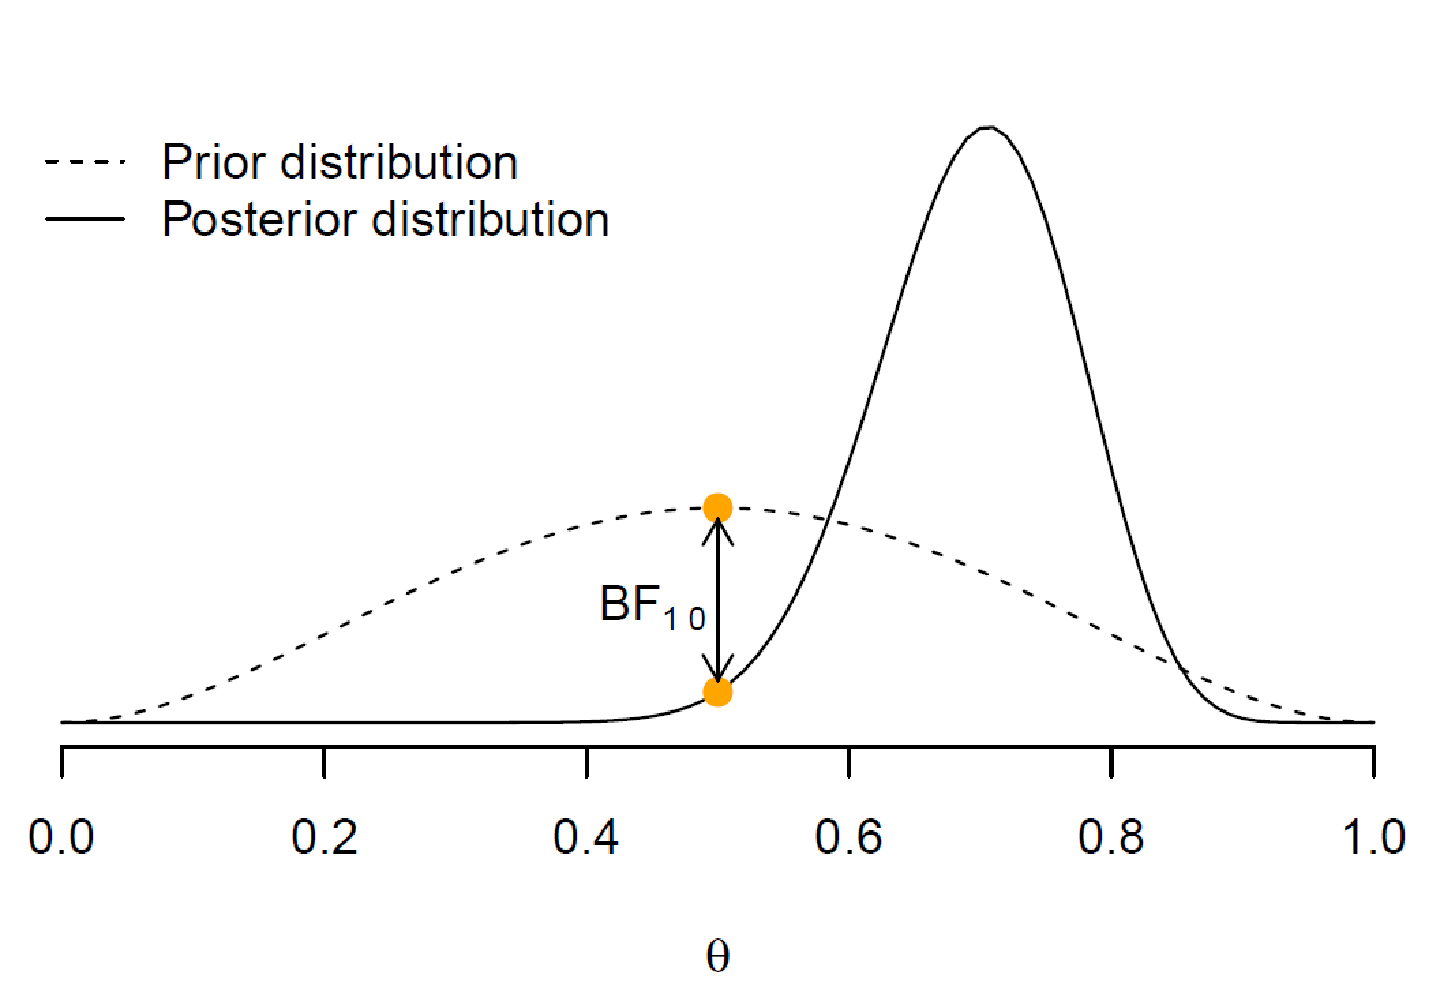
\includegraphics[width=0.8\textwidth]{Files/Images/priorAndPosterior.pdf}
\end{center}

\question{Use the \rcode{dbeta()} function to find out the height of your \concept{prior distribution} at the point $\theta = 0.5$ and store it in an object called \rcode{heightPrior}.}

\rcodeanswertiny

\question{Use the \rcode{dbeta()} function to find out the height of your \concept{posterior distribution} at the point $\theta = 0.5$ and store it in an object called \rcode{heightPosterior}.}

\rcodeanswertiny

\clearpage % Page break

Run the following code in \texttt{R} to compute the \concept{Bayes factor} in favor of the \concept{alternative hypothesis} $H_1$. \\
\\
\codeblock{BF10 <- heightPrior / heightPosterior}

\question{What is the value of the \concept{Bayes factor} \rcode{BF10}? Interpret this \concept{Bayes factor} with respect to the alternative hypothesis $H_1$.}

\twolineanswerbox

To make interpretation of the \concept{Bayes factor} more simple, the labels in the table below have been proposed. Please note that you shout not get too hung up on the specific labels and breakpoints in this table, since convincing evidence is different for every situation. \\

\begin{table}[h]
    \centering
    \begin{tabular}{r|l}
         Bayes factor & Evidence \\
         \hline
         1 - 3 & Anecdotal \\
         3 - 10 & Moderate \\
         10 - 30 & Strong \\ 
         30 - 100 & Very strong \\
         $>$ 100 & Extreme
    \end{tabular}
\end{table}

\question{Considering the labels from the table above, can you convincingly disprove the hypothesis that your algorithm makes a profitable trade with a probability other than if it were to trade stocks randomly?}

\twolineanswerbox

\question{Re-specify the $\alpha$ and $\beta$ parameters of the \concept{prior distribution} so that you express a different prior belief. Recalculate the \concept{Bayes factor} by running your code again. What is the new value of \rcode{BF10}. How robust in your \concept{Bayes factor} to changes in the prior distribution?}

\onelineanswerbox

\clearpage % Page break
\setcounter{chapter}{8}
\setcounter{section}{5}
\setcounter{question}{0}

%%%%%%%%%%%%%%%%%%%%%%%%%%%%%%%%%%%%%%%%%%%%%%%%%%%%%%%%%%%%%%%%%%%%%%%%%%%
% Assignment 8.5: Using bridge sampling to calculate the Bayes factor
%%%%%%%%%%%%%%%%%%%%%%%%%%%%%%%%%%%%%%%%%%%%%%%%%%%%%%%%%%%%%%%%%%%%%%%%%%%

\rassignment{Using bridge sampling to calculate the Bayes factor}

You are not convinced by the evidence from assignment 8.4 and want to perform additional testing. This time, however, you want to find out whether your algorithm makes more than 75 percent of the trades with profit. That is, you want to test whether $\theta$ is higher or lower than 0.75.\\

\question{Formulate the \concept{models} $M_1$ (restricts $\theta$ to be below 0.75) and $M_2$ (restricts $\theta$ to be higher than 0.75). Choose the restriction ($\leq$, $=$, or $\geq$) that applies to each model.}

\emptyanswerbox{
    $M_1$: $\theta \leq / = / \geq$ \tinyanswerline \hspace{3cm} $M_2$: $\theta \leq / = / \geq$ \tinyanswerline
}

For these more complicated (e.g., non-nested) models, the computation of the \concept{Bayes factor} becomes more difficult since it involves computing the \concept{marginal likelihoods} of the \concept{models}. To make your life simple, you can use the \rcode{bridgesampling} package together with the \rcode{rstan} package to let \texttt{R} calculate these values for you. \\

Run the following code in \texttt{R} to install the \rcode{bridgesampling} package. Then load the \rcode{bridgesampling} and the \rcode{rstan} package. \\
\\
\codeblock{install.packages(\textquotesingle bridgesampling\textquotesingle) \\
            \\
            library(bridgesampling) \\
            library(rstan)}

Copy and run the following code in \texttt{R} to set up the \texttt{Stan} model for $M_1$, the model that restricts $\theta$ to be lower than 0.75 and store it in an object called \rcode{model1}. The code then compiles the model using the \rcode{stan\_model()} function. \\
\\
\codeblock{model1code <- {\color{dataset}\textquotesingle} \\
{\color{dataset}data \{} \\
    \hspace*{20pt} {\color{dataset}int n;} \\
    \hspace*{20pt} {\color{dataset}int k;} \\
{\color{dataset}\}} \\
{\color{dataset}parameters \{ }\\
    \hspace*{20pt} {\color{dataset}real<lower=0,upper=0.75> theta; }\\
{\color{dataset}\}} \\
{\color{dataset}model \{ }\\
    \hspace*{20pt} {\color{dataset}theta {\raise.17ex\hbox{$\scriptstyle\sim$}} beta(1, 1)T[0, 0.75]; }\\
    \hspace*{20pt} {\color{dataset}k {\raise.17ex\hbox{$\scriptstyle\sim$}} binomial(n, theta); }\\
{\color{dataset} \} } \\
{\color{dataset}\textquotesingle} \\
\\
{\color{dataset}\# Note: The following line can take a while to execute}\\
model1 <- stan\_model(model\_code = model1code, model\_name = \textquotesingle model1\textquotesingle) }

\clearpage % Page break

\question{Create the \texttt{Stan} model for $M_2$, the model that restricts $\theta$ to be higher than 0.75, on the basis of the lines in \rcode{model1code}. Name the compiled model \rcode{model2}.}

\hint{First find out what elements were added to the code since assignment 8.3.}

\rcodeanswerlarge

\question{Locate and describe the \concept{prior distributions} for $\theta$ in $M_1$ and $M_2$.}

\twolineanswerbox

Now you start collecting data again. Suppose that you monitor your algorithm for $n = 156$ more trades, and find that $k = 123$ trades resulted in a profit. \\

\question{Use the \rcode{sampling()} function to sample for the \concept{models} $M_1$ and $M_2$ using these data. Store the fitted \texttt{Stan} models in objects named \rcode{stanFitM1} and \rcode{stanFitM2}.}

\rcodeanswersmall

\question{Use the \rcode{bridge\_sampler()} function to calculate the \concept{marginal likelihoods} of the models $M_1$ and $M_2$ and store them in \rcode{mLike1} and \rcode{mLike2}.}

\rcodeanswersmall

\clearpage % Page break

\question{Use the \rcode{bf()} function to calculate the \concept{Bayes factor} $BF_{21}$ in favor of model $M_2$ over model $M_1$ and store it in an object called \rcode{BF21}.}

\hint{Be sure to insert the two marginal likelihoods into the \rcode{bf()} function in the correct order so that the result is $BF_{21}$.}

\question{What is the value of \rcode{BF21}? Interpret this \concept{Bayes factor} with respect to the model that restricts $\theta$ to be higher than 0.75.}

\threelineanswerbox

\question{What is the strength of evidence associated with this \concept{Bayes factor}? Are you convinced by this evidence?}

\threelineanswerbox

\clearpage % Page break